%!TEX root = thesis.tex
\chapter{Results}\label{chap:results}
\thispagestyle{plain}

% ==== SECTION 1 ===============================================================
\section{Equilibrium experiments} % (fold)
\label{sec:equilibrium_experiments_results}
    Equilibrium experiment are a useful tool to asses the behavior of glacier models. The OGGM provides two climate scenarios for such equilibrium experiment, the \lstinline`ConstantMassBalance` model and the \lstinline`RandomMassBalance` model. The implementation and workings of both mass balance models are described in Subsection~\ref{sub:mass_balance_models_implementation}.

    The experiments are performed on all alpine glaciers using the HISTALP dataset \citep{Auer2007} as climatic input data. The baseline climate for each glacier comes from a 31-year period centered around the \textit{equilibrium year} \tstar. An additional temperature bias of \SI{0}{\celsius}, \SI{-0.5}{\celsius} and \SI{+0.5}{\celsius} results in a neutral, positive and negative step change in mass balance, respectively. The detailed experimental setup can be found in Section~\ref{sub:equilibrium_experiments_setup}

    The first qualitative conclusions are drawn from the temporal evolution of glacier length, surface area and ice volume. We are looking at selected single glaciers as well as at the regional scale, i.e. at the sum over all glaciers in the HISTALP domain. Scaling methods applied to a single glacier give only an order of magnitude estimation \citep[section 8.5][cf.]{Bahr2015}, which is accounted for in the following analysis. More quantitative results are drawn from an autocorrelation analysis and a power spectral density analysis, inspired by \citet{Roe2014}.
    
    \subsection{Time series} % (fold)
    \label{sub:time_series_results}

      The following section tries to explain the model behavior using the temporal evolution of the glacier length, surface area and ice volume. The plots show a comparison between the \vas{} model and the flowline model time series, both for the constant and random climate scenario. Since the \vas{} model derives the initial glacier geometry from the surface area, absolute values of initial length and volume differ between the \vas{} model and the flowline model. The results are therefore normalized with respect to their initial values for better comparability. 

      \subsubsection*{Overall findings}

      \begin{itemize}
        \item Both evolution models behave as expected and produce the same qualitative results. The model glaciers stay in an approximate equilibrium state using the climate around \tstar and decreases/increases in size (length, area, volume) for a positive/negative temperature bias. Plots with absolute values can be found in the appendix % TODO
        \item The glacier size (length, area, volume) changes drastically less (i.e., between two to eight times less) with the \vas{} model than with the flowline model.
        However, volume estimations from volume/area scaling of a single glaciers must be considered as order of magnitude result. The scaling constant $c$ is a random variable which can vary drastically from glacier to glacier. Apparently, the global mean value of $c=0.034\ \mathrm{km^{3-2\gamma}}$ is a bad fit for the characteristics of Hintereisferner.
      \end{itemize}
      

      1. 

      2. The glacier size changes (dramatically) less under the VAS model than under the flowline model (true for length, area, and volume).

         *Note*: However, volume estimations from volume/area scaling of a single glaciers must be considered as order of magnitude result. The scaling constant $c$ is a random variable which varies (drastically) from glacier to glacier. Apparently, the global mean value of $c=0.034\ \mathrm{km^{3-2\gamma}}$ is a bad fit for the characteristics of Hintereisferner.

         *Second Note*: Changing the scaling constants changes the absolute values of ice volume (as well as surface area and glacier length). A higher volume/area scaling constant results in a larger initial ice volume. Subjected to the same climate perturbation (temperature step change), an initially larger glacier will gain/loose more ice and reach a higher equilibrium ice volume than a smaller one. However, when normalized with initial ice volume there are no more discernible differences in the magnitude of ice volume change. The temporal evolution, i.e., the oscillation behavior, is comparable, even if smaller glaciers react faster than larger ones (which is to be expected).

         *TL;DR; Turns out, the scaling constant does not change the magnitude of the normalized volume change.* 

      3. The glacier length of the VAS model has to be seen more as a model parameter, rather than as an actual glacier property. The VAS glacier length decreases/increases only by about 8 percent compared to its initial value, for a positive/negative temperature bias of 0.5 °C. This correspond to an absolute length change of less than 400 m, which is very little compared to the 3 to 4 km in length change (~40% of the initial value) produced by the flowline model. (*Note*: May change with different $c$ parameter. *Second note*: Turns out, it does not when normalized with initial length.)

      4. The result of VAS model under a constant climate scenario with a non-zero temperature bias reminds of a damped oscillating signal. The modeled length reaches its maximum after ~200 years, overshooting the equilibrium result by more than 1%. Followed by two minor but still discernible peaks until the new equilibrium is reached. Both, glacier surface area and glacier volume reach their maximum earlier and overshoot by more.
    
    % subsection time_series (end)

    \subsection{Constant climate scenario} % (fold)
    \label{sub:constant_climate_scenario_results}

    
    % subsection constant_climate_scenario (end)

    \subsection{Random climate scenario} % (fold)
    \label{sub:random_climate_scenario_results}
    
    % subsection random_climate_scenario (end)

    \subsection{Autocorrelation analysis} % (fold)
    \label{sub:autocorrelation_analysis_results}

      The autocorrelation function for selected glaciers is shown in Figure~\ref{fig:acf}. For details about the experimental setup see Section~\ref{ssub:autocorrelation_analysis_setup}

      The autocorrelation function of the \vas{} length shows little to no variability between runs under different climate conditions. % TODO compare with almost linear behavior of mass balance model in the vicinity of equilibirum
      The autocorrelation function of the \vas{} length is comparable even between different glaciers. It has the same behavior of a dampened oscillator as described above. Their are differences in amplitude and frequency--most likely affected by glacier size--the general behavior is almost identical. 
      
      The flowline model is able to represent different glacial geometries and grasp individual responses to climatic forcings, which can be seen in the vastly different autocorrelation functions. They differ from glacier to glacier, but also for different climate scenarios (temperature biases) on the same glacier. However, there are no discernible patterns, which again confirms the notion that the OGGM flowline model is capable of modeling each glaciers individual response. Here are some examples: for Hintereisferner the autocorrelation of the flowline model is stronger than that of the \vas{} model, while for Mer de Glace and Großer Aletschgletscher it is lower (for all tested climate scenarios); the flowline model of the Pasterze shows a strong autocorrelation under the equilibrium climate, i.e., \SI{0}{\celsius} temperature bias, (>0.7 for lags times between 0 and 95 years, still >0.43 for 200 years lag time, statistically significant up until a lag time of 232 years), while with a positive and negative temperature bias of \SI{\pm0.5}{\celsius} the autocorrelation is less than for the \vas{} model.
      The \vas{} model has a stronger autocorrelation for short lag time (i.e., less than about 20 years) than the flowline model; similarly, the flowline model of the Glacier d'Argentière shows a strong autocorrelation under the climate with \SI{+0.5}{\celsius} temperature bias, and lower autocorrelation than the \vas{} model for the other two climate scenarios; The only observation made for all glaciers, it that the \vas{} model has a stronger autocorrelation for short lag time (i.e., less than about 20 years) than the flowline model. This is true even for glaciers, where the autocorrelation of the flowline mode is generally stronger (e.g., Hintereisferner). 

      It is not the intent of this work to investigate the relation between a glacier's geometry and its autocorrelation function, therefore we leave it at this qualitative first look. However, it is notable that the OGGM flowline model behaves differently for different glaciers and/or different climatic forcings. How far these results are comparable to real world glaciers is anyones guess. The \textit{one size fits all} approach of the \vas{} model produces comparable results, mostly independent the glaciers geometry and the climate forcing (which was to be expected).


      \begin{figure}[htp]
        \centering
        \begin{subfigure}[b]{0.48\textwidth}
          \caption{RGI60-11.00897 - Hintereisferner}
          \label{fig:acf:hintereisferner}
          \centering
          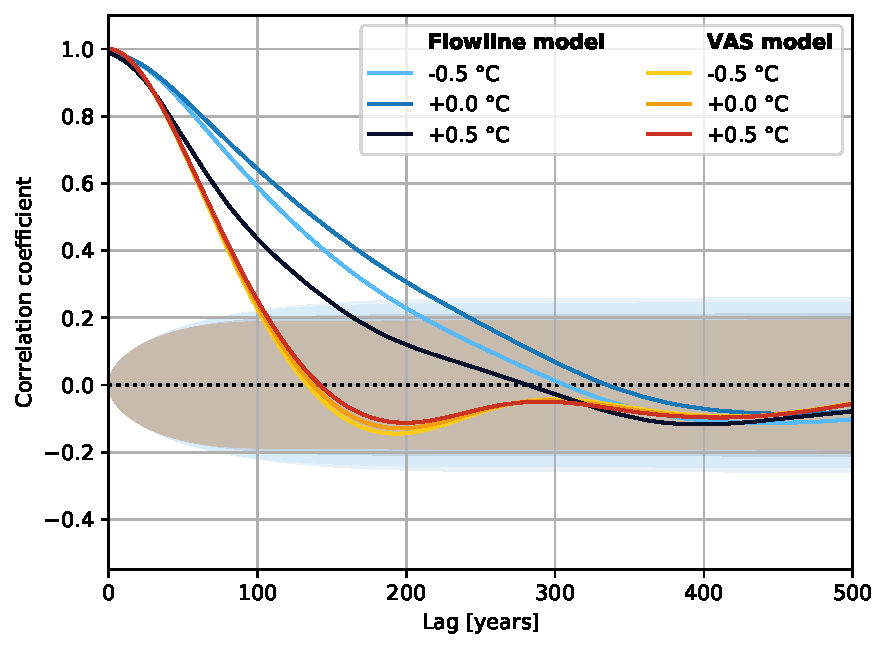
\includegraphics[width=\textwidth]{../plots/final_plots/acf/Hintereisferner.pdf}
        \end{subfigure}
        \hfill
        \begin{subfigure}[b]{0.48\textwidth}
          \caption{RGI60-11.00106 - Pasterze}
          \label{fig:acf:pasterze}
          \centering
          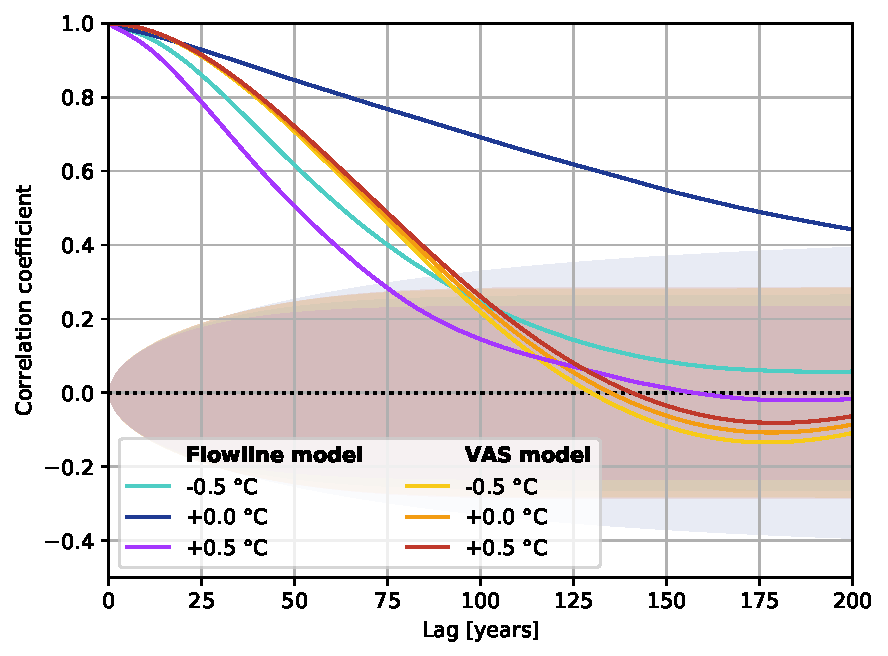
\includegraphics[width=\textwidth]{../plots/final_plots/acf/Pasterze.pdf}
        \end{subfigure}
        \begin{subfigure}[b]{0.48\textwidth}
          \caption{RGI60-11.03643 - Mer de Glace}
          \label{fig:acf:mer_de_glace}
          \centering
          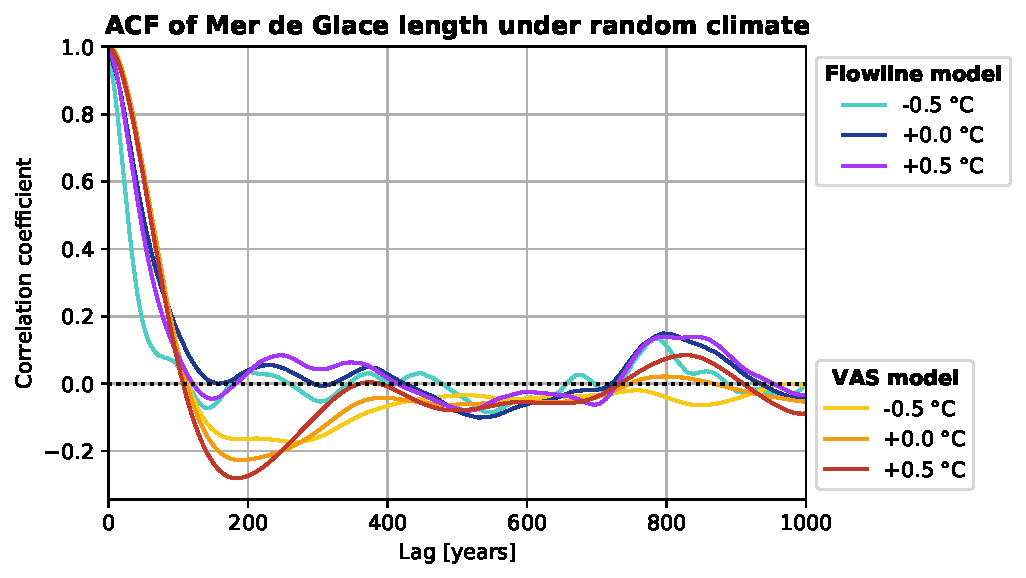
\includegraphics[width=\textwidth]{../plots/final_plots/acf/Mer_de_Glace.pdf}
        \end{subfigure}
        \hfill
        \begin{subfigure}[b]{0.48\textwidth}
          \caption{RGI60-11.03638 - Glacier d'Argentière}
          \label{fig:acf:glacier_d_argentiere}
          \centering
          \includegraphics[width=\textwidth]{../plots/final_plots/acf/Glacier_d'Argentière.pdf}
        \end{subfigure}
        \begin{subfigure}[b]{0.48\textwidth}
          \caption{RGI60-11.01450 - Großer Aletschgletscher}
          \label{fig:acf:großer_aletschgletscher}
          \centering
          \includegraphics[width=\textwidth]{../plots/final_plots/acf/Großer_Aletschgletscher.pdf}
        \end{subfigure}
        \hfill
        \begin{subfigure}[b]{0.48\textwidth}
          \caption{RGI60-11.01238 - Rhonegletscher}
          \label{fig:acf:rhonegletscher}
          \centering
          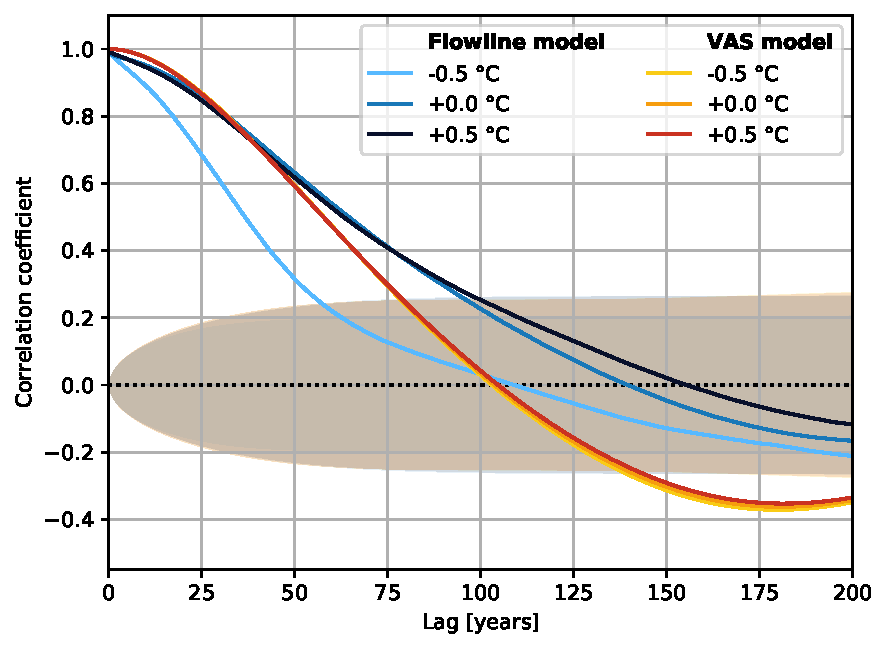
\includegraphics[width=\textwidth]{../plots/final_plots/acf/Rhonegletscher.pdf}
        \end{subfigure}
        % \begin{subfigure}[b]{0.48\textwidth}
        %   \caption{RGI60-11.02704 - Allalingletscher}
        %   \label{fig:acf:allalingletscher}
        %   \centering
        %   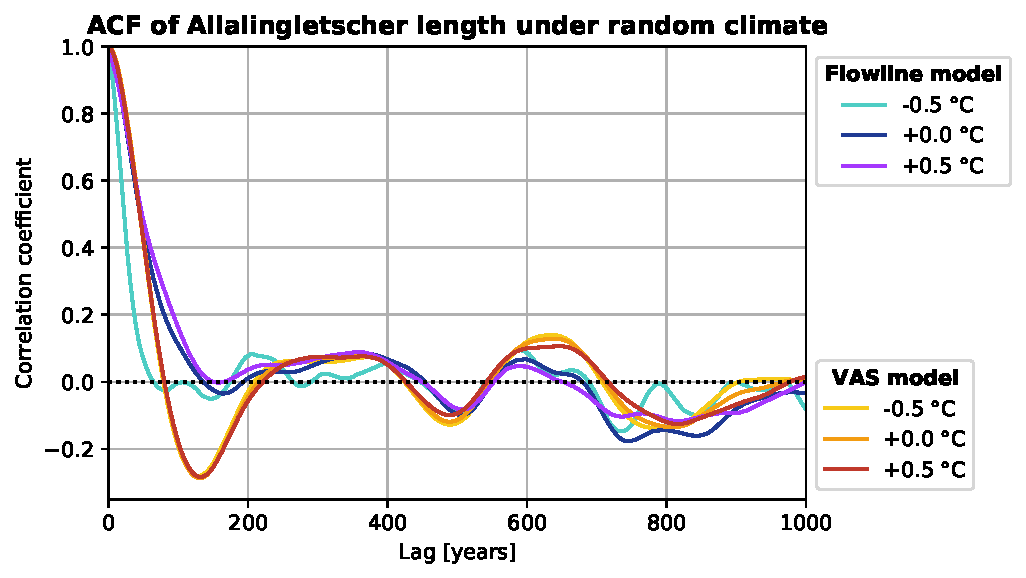
\includegraphics[width=\textwidth]{../plots/final_plots/acf/Allalingletscher.pdf}
        % \end{subfigure}
        % \hfill
        % \begin{subfigure}[b]{0.48\textwidth}
        %   \caption{RGI60-11.02773 - Findelgletscher}
        %   \label{fig:acf:findelgletscher}
        %   \centering
        %   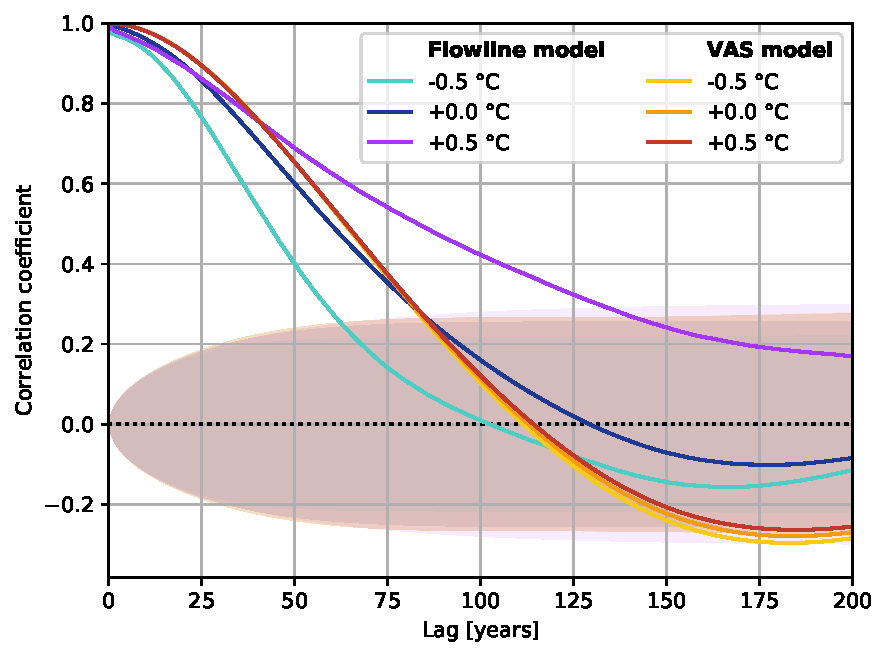
\includegraphics[width=\textwidth]{../plots/final_plots/acf/Findelgletscher.pdf}
        % \end{subfigure}

        \caption{Autocorrelation function of modeled glacier length for lag times between zero and 200 years. Different lines represent different combinations of evolution model and climate scenario.
        The random climate scenario is based on an equilibrium climate, with different temperature biases.
        Cyan, blue and purple lines represent the flowline model, while yellow, orange and red lines represent the \vas{} model, with a temperature bias of \SI{-.5}{\celsius}, \SI{0}{\celsius} and \SI{+.5}{\celsius}, respectively.
        The \SI{99}{\percent} confidence intervals are shaded in the corresponding colors.}
        \label{fig:acf}
      \end{figure}
    
    % subsection sub:autocorrelation_analysis_results (end)

% section equilibrium_experiments (end)

% ==== SECTION 2 ===============================================================
\section{Sensitivity experiments} % (fold)
\label{sec:sensitivity_experiments_results}

% section sensitivity_experiments (end)

% ==== SECTION 3 ===============================================================
\section{Future projection} % (fold)
\label{sec:future_projection_results}

% section future_projection (end)